\documentclass[week3]{csse2002}
\usepackage{slides}

\usepackage{tikz}
\usetikzlibrary{positioning}

\author{Brae Webb}

\title{CSSE2002 Week 3 Tutorial}
 
\begin{document}

\begin{frame}
\maketitle
\end{frame}

\begin{topic}{Admin}
\begin{enumerate}
    \item Attend lectures!
    \item Version Control practical task
    \item Assignment release
\end{enumerate}
\end{topic}

\begin{topic}{This Week...}
\begin{enumerate}
    \item Classes (a refresher)
    \item Interfaces
    \item Inheritance
    \item Casting
\end{enumerate}
\end{topic}

\begin{topic}{Class Diagram}
\begin{java}
public class Animal {}
public class Lion extends Animal {}
public class Dog extends Animal implements Pet {}
public class Poodle extends Dog {}
public interface Pet {}
\end{java}
\begin {tikzpicture}[-latex ,auto ,node distance =2 cm and 5cm ,on grid ,
semithick ,
state/.style ={ circle ,top color =white , bottom color = processblue!20 ,
draw,processblue , text=blue , minimum width =0 cm}]
\node[state] (A) {Animal};
\node[state] (B) [below right=of C] {Dog};
\node[state] (E) [below left=of C] {Lion};
\node[state] (D) [below=of B] {Poodle};
\node[state] (C) [right =of C] {Pet};
\path (B) edge [left] node[left] {} (A);
\path (D) edge [left] node[left] {} (B);
\path (E) edge [left] node[left] {} (A);
\path [dashed] (C) edge [left] node[left] {} (B);
\end{tikzpicture}
\end{topic}

% \begin{topic}{Motitivation}
% 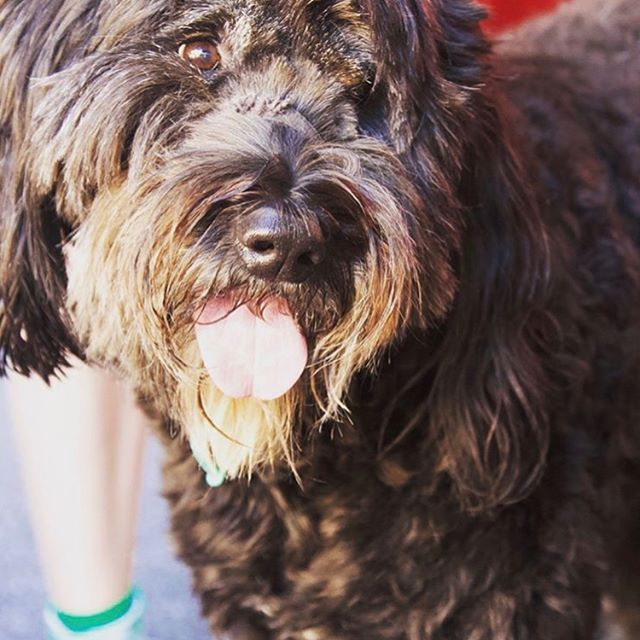
\includegraphics[width=\textwidth,keepaspectratio]{doggo.jpg}
% \end{topic}

\begin{topic}{Casting}
\begin{subtopic}{1-}
\begin{enumerate}
	\item To cast from one class to another class, the classes need some relation (i.e. on the same branches of the class hierarchy)
	\item 'Up-casts' allow casts to be implicit (widening of scope / more general)
	\item 'Down-casts' require that casts are explicit (narrowing of scope / more specific)
	\item 'Down-casts' can cause \emph{runtime errors}
\end{enumerate}
\end{subtopic}

\begin{subtopic}{2-}
\begin{java}
public class Animal {}
public class Lion extends Animal {}
public class Dog extends Animal implements Pet {}
public class Poodle extends Dog {}
public interface Pet {}

Dog evie = new Dog();
Animal animal = (Animal) evie; // can be implicit
// Animal animal = evie;
Lion mufasa = (Lion) animal; // has to be explicit
Dog harlee = (Dog) animal; // still has to be explicit
\end{java}
\end{subtopic}
\end{topic}

\begin{topic}{Poll}
\begin{subtopic}{1-}
\begin{java}
public class Animal {}
public class Lion extends Animal {}
public class Dog extends Animal implements Pet {}
public class Poodle extends Dog {}
public interface Pet {}
\end{java}
\end{subtopic}

\begin{subtopic}{2-}
\begin{java}
Dog evie = new Dog();
Animal animal = evie;
Dog harlee = animal;
\end{java}
\end{subtopic}

\begin{subtopic}{3-}
\begin{java}
Dog evie = new Dog();
Animal animal = (Animal) evie;
Lion mufasa = (Lion) animal;
\end{java}
\end{subtopic}
\end{topic}

% \begin{topic}{Discussion \& More Motivation}
% 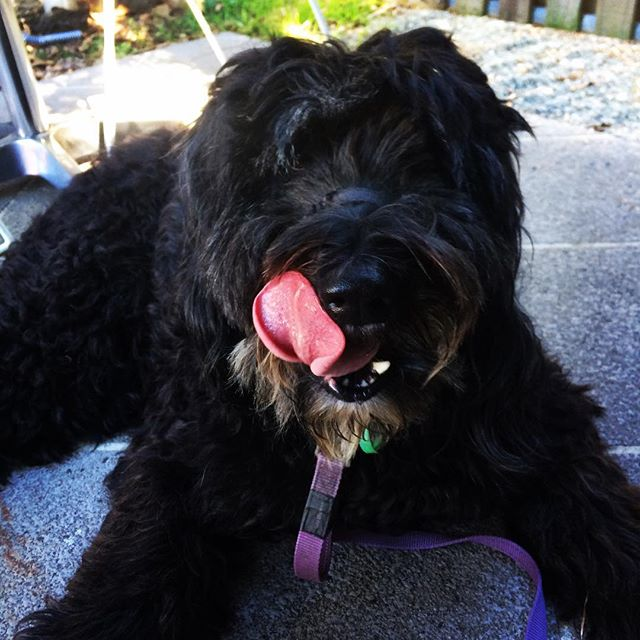
\includegraphics[width=\textwidth,keepaspectratio]{doggo2.jpg}
% \end{topic}

\begin{topic}{Runtime vs Compile-time}
\begin{subtopic}{1-}

Compile-time is what you tell the compiler

Runtime is the actual type

\begin{java}
Animal animal = new Dog();
\end{java}
\end{subtopic}

\begin{subtopic}{2-}
\texttt{Animal} is the compile-time or static type

\texttt{Dog} is the runtime or dynamic type
\end{subtopic}
\end{topic}

\begin{topic}{Method Signature}
In java the signature of a method is defined as the following:
\begin{enumerate}
	\item The method name
	\item The method parameters (amount, type and order NOT name)
\end{enumerate}

\begin{java}
public int add(int x, double y);
// The method name: add
// The method parameters: int, double
// Signature: add(int, double)
\end{java}
\end{topic}

\begin{topic}{Method Resolution}
When a method is called on a variable the following steps are used to determine
which method to actually call:
\begin{enumerate}
	\item The static type of the variable is used to determine the method signature
	\item The dynamic (or runtime) type of the variable is used to lookup a class
	\item If the dynamic type doesn't have the method defined, traverse inheritance hierarchy
\end{enumerate}

\begin{java}
public class Animal {
	public void eat() {}
}
public class Dog extends Animal {
	public void eat() {}
}
public class Poodle extends Dog {}

Animal evie = new Poodle();
evie.eat();
\end{java}
\end{topic}

\end{document} 
